\newcommand{\lecturetitle}[1]{
  \title{01204211 Discrete Mathematics \\ #1}
  \author{Jittat Fakcharoenphol}
  \frame{\titlepage}
}

\lecturetitle{Lecture 8: Mathematical Induction 3}

\begin{frame}\frametitle{Review: Mathematical Induction}
  \begin{tcolorbox}
    Suppose that you want to prove that property $P(n)$ is true for
    every natural number $n$.\\
    
    Suppose that we can prove the following two facts:
    
    {\bf Base case:} $P(1)$ \\
    {\bf Inductive step:} For any $k\geq 1$, $P(k)\Rightarrow P(k+1)$ \\
    
    The {\bf Principle of Mathematical Induction} states that $P(n)$
    is true for every natural number $n$.
  \end{tcolorbox}

  The assumption $P(k)$ in the inductive step is usually referred to
  as {\bf the Induction Hypothesis}.
\end{frame}

\begin{frame}\frametitle{The Induction Hypothesis}
  \begin{theorem}
    For any integer $n\geq 1$, $\frac{1}{1^2} + \frac{1}{2^2} + \frac{1}{3^2} + \cdots +\frac{1}{n^2} < 2$.
  \end{theorem}
  \pause
  \begin{proof}
    The statement $P(n)$ that we want to prove is ``$\frac{1}{1^2} + \frac{1}{2^2} + \frac{1}{3^2} + \cdots +\frac{1}{n^2} < 2$''.
    
    \pause
    \vspace{0.1in}

    {\bf Case case:} For $n=1$, the statement is true because $1<2$.

    \pause
    \vspace{0.1in}
    
    {\bf Inductive step:} For $k\geq 1$, let's assume $P(k)$ and we prove that $P(k+1)$ is true.

    \pause

    The induction hypothesis is: $\frac{1}{1^2} + \frac{1}{2^2} + \frac{1}{3^2} + \cdots +\frac{1}{k^2} < 2$.

    We want to show $P(k+1)$, i.e., $\frac{1}{1^2} + \frac{1}{2^2} + \frac{1}{3^2} + \cdots +\frac{1}{k^2}+\frac{1}{(k+1)^2} < 2$.

    Then...
  \end{proof}
\end{frame}

\begin{frame}\frametitle{Strengtening the Induction Hypothesis (1)}
  \begin{itemize}
  \item
    Is the assumption
    \[ \frac{1}{1^2} + \frac{1}{2^2} + \frac{1}{3^2} + \cdots +\frac{1}{k^2} < 2.\]
    ``strong'' enough to prove
    \[ \frac{1}{1^2} + \frac{1}{2^2} + \frac{1}{3^2} + \cdots +\frac{1}{k^2}+\frac{1}{(k+1)^2} < 2 \ \ ?\]

    Why?
    \pause
    
  \item To prove $P(k+1)$, we need a ``gap'' between the LHS and 2, so
    that we can add $1/(k+1)$ without blowing up the RHS.
  \end{itemize}
\end{frame}

\begin{frame}\frametitle{Strengtening the Induction Hypothesis (2)}
  \begin{itemize}
  \item Let's see a few values of the sum:
    \begin{itemize}
    \item $1/1 = 1.$ \pause
    \item $1/1 + 1/4 = 1.25.$ \pause
    \item $1/1 + 1/4 + 1/9 \approx 1.361.$ \pause
    \item $1/1 + 1/4 + 1/9 + 1/16 \approx 1.4236.$ \pause
    \item $1/1 + 1/4 + 1/9 + 1/16 + 1/25 \approx 1.4636.$
    \end{itemize}
    Yes, there is a gap.  But how large?
    \pause
    
  \item We need the gap to be large enough to insert $1/(k+1)^2$.
    \pause
  \item After a ``mysterious'' moment, we observe that
    \[ \frac{1}{1^2} + \frac{1}{2^2} + \frac{1}{3^2} + \cdots +\frac{1}{n^2} < 2 - \frac{1}{n}.\]
  \end{itemize}
\end{frame}

\begin{frame}\frametitle{Strengtening the Induction Hypothesis (3)}
  \begin{theorem}
    For any integer $n\geq 1$, $\frac{1}{1^2} + \frac{1}{2^2} + \frac{1}{3^2} + \cdots +\frac{1}{n^2} < 2 - \frac{1}{n}$.
  \end{theorem}
  \pause
  \begin{proof}
    {\footnotesize
      (... the beginning is left out ...)
      
      {\bf Inductive step:} For $k\geq 1$, assume that $ \frac{1}{1^2} + \frac{1}{2^2}  + \cdots +\frac{1}{k^2} < 2 - \frac{1}{k}. $
      
      Adding $1/(k+1)^2$ on both sides, we get
      \[ \frac{1}{1^2} + \frac{1}{2^2}  + \cdots +\frac{1}{k^2}+\frac{1}{(k+1)^2}
      < 2 - \frac{1}{k} +\frac{1}{(k+1)^2}
      = 2 - \left(\frac{1}{k} - \frac{1}{(k+1)^2}\right).\]

     Since $1/k - 1/(k+1) = 1/(k(k+1))$, we have that
      \[1/(k+1) = 1/k - 1/(k(k+1)) < 1/k - 1/(k+1)^2.\]

      Therefore, we conclude that
      \[
      \frac{1}{1^2} + \frac{1}{2^2} + \cdots +\frac{1}{k^2}+\frac{1}{(k+1)^2}
      < 2 - \left(\frac{1}{k} - \frac{1}{(k+1)^2}\right)
      < 2 - \frac{1}{k+1},
      \]
      as required.
    }
  \end{proof}
\end{frame}

\begin{frame}\frametitle{A Lesson learned}
  \begin{itemize}
  \item
    Is a stronger statement easier to prove?
    \pause
  \item
    In this case, the statement is indeed stronger, but the induction
    hypothesis gets stronger as well.  Sometimes, this works out
    nicely.
  \end{itemize}
\end{frame}

\begin{frame}\frametitle{L-shaped tiles (1)}
  A 4x4 area with a hole in the middle can be tiled with L-shaped tiles.

  \vspace{0.2in}
  
  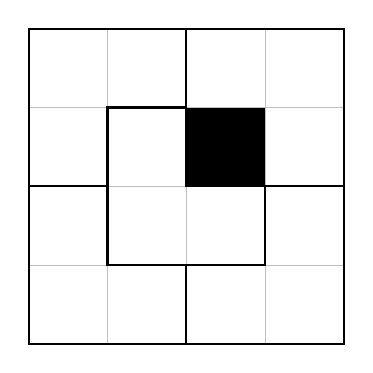
\begin{tikzpicture}
    \draw[step=1cm,lightgray,ultra thin] (0,0) grid (4,4);
    \fill[black] (2,2) -- (2,3) -- (3,3) -- (3,2) -- cycle;
    \draw[thick] (0,0) -- (0,2) -- (1,2) -- (1,1) -- (2,1) -- (2,0) -- cycle;
    \draw[thick] (0,2) -- (0,4) -- (2,4) -- (2,3) -- (1,3) -- (1,2) -- cycle;
    \draw[thick] (1,1) -- (1,3) -- (2,3) -- (2,2) -- (3,2) -- (3,1) -- cycle;
    \draw[thick] (2,2) rectangle (4,4);
    \draw[thick] (4,2) -- (4,0) -- (2,0);
  \end{tikzpicture}
\end{frame}

\begin{frame}\frametitle{L-shaped tiles (2)}
  This is true for 2x2 area, 8x8 area, even 16x16 area.
  \vspace{0.1in}

  
\begin{tikzpicture}
    \draw[step=0.5cm,lightgray,ultra thin] (0,0) grid (1,1);
    \fill[black] (0.5,0.5) -- (1,0.5) -- (1,1) -- (0.5,1) -- cycle;
  \end{tikzpicture}
  \ \ 
  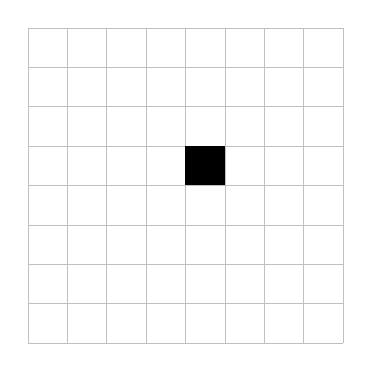
\begin{tikzpicture}
    \draw[step=0.5cm,lightgray,ultra thin] (0,0) grid (4,4);
    \fill[black] (2,2) -- (2,2.5) -- (2.5,2.5) -- (2.5,2) -- cycle;
  \end{tikzpicture}  
  \ \
  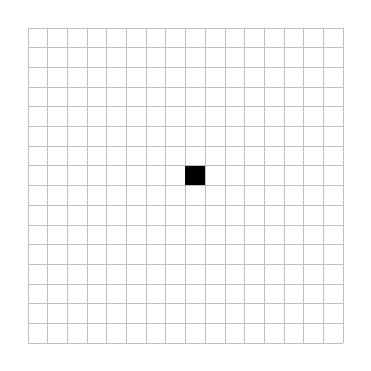
\begin{tikzpicture}
    \draw[step=0.25cm,lightgray,ultra thin] (0,0) grid (4,4);
    \fill[black] (2,2) -- (2,2.25) -- (2.25,2.25) -- (2.25,2) -- cycle;
  \end{tikzpicture}  
  
  \vspace{0.1in}

  This motivates us to try to prove that it is possible to use
  L-shaped tiles to tile a $2^n\times 2^n$ area.
\end{frame}

\begin{frame}\frametitle{Proving the fact?}
  \begin{theorem}
    For integer $n\geq 1$, an area of size $2^n\times 2^n$ with one
    hole in the middle can be tiled with L-shaped tiles.
  \end{theorem}
  \textcolor{blue}{Proof:}  We prove by induction on $n$.
  
  {\bf Base case:} For $n=1$, $2^1\times 2^1$ area with a hole in
  the middle can be tiled.

  {\bf Inductive step:} Assume that for $k\geq 1$, an $2^k\times
  2^k$ area with a hole in the middle can be tiled.  We shall prove
  the statement for $n=k+1$, i.e., that an $2^{k+1}\times 2^{k+1}$
  area with one hole in the middle can be tiled.
  
  (cont. on the next page)
\end{frame}

\begin{frame}\frametitle{Proving the fact?}
  \textcolor{blue}{Proof: (cont.)}

  Let's see the Induction Hypothesis and the goal:
    
  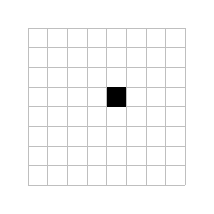
\begin{tikzpicture}
    \draw[step=0.25cm,lightgray,ultra thin] (0,0) grid (2,2);
    \fill[black] (1,1) -- (1,1.25) -- (1.25,1.25) -- (1.25,1) -- cycle;
  \end{tikzpicture}  
  \ \
  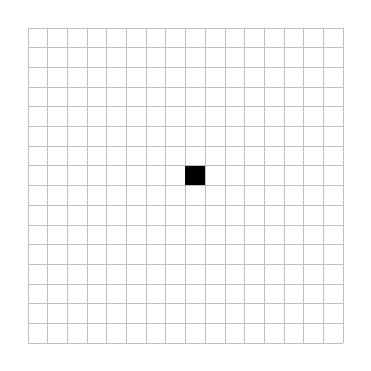
\begin{tikzpicture}
    \draw[step=0.25cm,lightgray,ultra thin] (0,0) grid (4,4);
    \fill[black] (2,2) -- (2,2.25) -- (2.25,2.25) -- (2.25,2) -- cycle;
  \end{tikzpicture}  
  \ \ \pause
  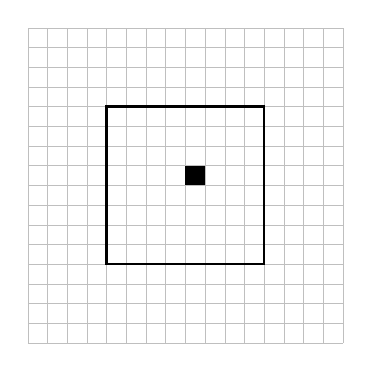
\begin{tikzpicture}
    \draw[step=0.25cm,lightgray,ultra thin] (0,0) grid (4,4);
    \fill[black] (2,2) -- (2,2.25) -- (2.25,2.25) -- (2.25,2) -- cycle;
    \draw[thick] (1,1) rectangle (3,3);
  \end{tikzpicture}  
  
  With the current form of the Induction Hypothesis, this is
  probably the way to use it.  \pause But it seems hard to go
  further with this approach....
\end{frame}

\begin{frame}\frametitle{Let's try a different approach}
  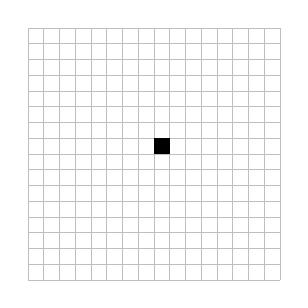
\begin{tikzpicture}[scale=0.8]
    \draw[step=0.25cm,lightgray,ultra thin] (0,0) grid (4,4);
    \fill[black] (2,2) -- (2,2.25) -- (2.25,2.25) -- (2.25,2) -- cycle;
  \end{tikzpicture}
  \ \ \pause
  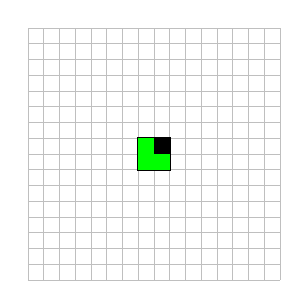
\begin{tikzpicture}[scale=0.8]
    \draw[step=0.25cm,lightgray,ultra thin] (0,0) grid (4,4);
    \draw[thick] (1.75,1.75) rectangle (2.25,2.25);
    \fill[green] (1.75,1.75) rectangle (2.25,2.25);
    \fill[black] (2,2) -- (2,2.25) -- (2.25,2.25) -- (2.25,2) -- cycle;
  \end{tikzpicture}
  \ \ \pause
  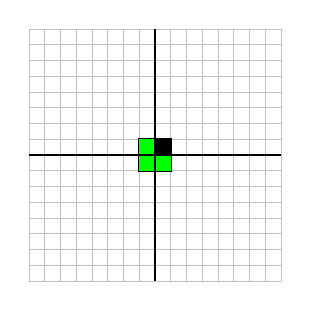
\begin{tikzpicture}[scale=0.8]
    \draw[step=0.25cm,lightgray,ultra thin] (0,0) grid (4,4);
    \draw[thick] (1.75,1.75) rectangle (2.25,2.25);
    \fill[green] (1.75,1.75) rectangle (2.25,2.25);
    \fill[black] (2,2) -- (2,2.25) -- (2.25,2.25) -- (2.25,2) -- cycle;
    \draw[thick] (0,2) -- (4,2);
    \draw[thick] (2,0) -- (2,4);
  \end{tikzpicture}
  \pause

  The last step seems nice, because it shows how we can solve the
  problem in the $2^{k+1}\times 2^{k+1}$ area with 4 problems in the
  $2^k\times 2^k$ areas.  \pause But do you see an issue with this
  approach regarding the Induction Hypothesis? \pause

  {\bf Current Inductive Hypothesis:} Assume that for $k\geq 1$, an
  $2^k\times 2^k$ area with ``a hole in the middle'' can be tiled.
  \pause
  
  {\bf A Stronger Inductive Hypothesis:} Assume that for $k\geq 1$, an
  $2^k\times 2^k$ area with {\textcolor{blue}{one hole}} can be tiled.
\end{frame}

\begin{frame}\frametitle{A stronger statement}
  \textcolor{blue}{Theorem:} For integer $n\geq 1$, an area of size
  $2^n\times 2^n$ with one hole can be tiled with L-shaped tiles.

  \textcolor{blue}{Proof:} We prove by induction on $n$.

  {\bf Base case:} For $n=1$, $2^1\times 2^1$ area with one hole can
  be tiled; \pause there are 4 cases shown below.

  \vspace{0.1in}
  
  
\begin{tikzpicture}
    \draw[step=0.5cm,lightgray,ultra thin] (0,0) grid (1,1);
    \fill[black] (0.5,0.5) -- (1,0.5) -- (1,1) -- (0.5,1) -- cycle;
  \end{tikzpicture}  
  \ \
  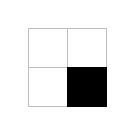
\begin{tikzpicture}
    \draw[step=0.5cm,lightgray,ultra thin] (0,0) grid (1,1);
    \fill[black] (0.5,0.5) -- (1,0.5) -- (1,0) -- (0.5,0) -- cycle;
  \end{tikzpicture}  
  \ \
  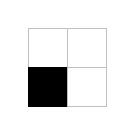
\begin{tikzpicture}
    \draw[step=0.5cm,lightgray,ultra thin] (0,0) grid (1,1);
    \fill[black] (0.5,0.5) -- (0,0.5) -- (0,0) -- (0.5,0) -- cycle;
  \end{tikzpicture}  
  \ \
  
\begin{tikzpicture}
    \draw[step=0.5cm,lightgray,ultra thin] (0,0) grid (1,1);
    \fill[black] (0.5,0.5) -- (0,0.5) -- (0,1) -- (0.5,1) -- cycle;
  \end{tikzpicture}  

  \pause
  
  {\bf Inductive step:} Assume that for $k\geq 1$, an $2^k\times
  2^k$ area with one hole can be tiled.  We shall prove
  the statement for $n=k+1$, i.e., that an $2^{k+1}\times 2^{k+1}$
  area with one hole can be tiled.
  \pause
  
  (Try to finish it in homework.)
\end{frame}

\begin{frame}\frametitle{Proof of the Principle of Mathematical Induction}
  \begin{theorem}
    If $P(1)$ and for any integer $k\geq 1$, $P(k)\Rightarrow P(k+1)$,
    then $P(n)$ for all natural number $n$.
  \end{theorem}
  \begin{proof}
    \pause We prove by contradiction.  \pause Assume that $P(n)$ is
    not true for some natural number $n$.  \pause Let $m$ be the
    smallest positive integer such that $P(m)$ is false.  \pause If
    $m=1$, we get a contradiction because we know that $P(1)$ is true;
    therefore, we know that $m>1$. \pause
 
    Since $m$ is smallest and $m > 1$, then $P(m-1)$ must be
    true. \pause However, because for any integer $k\geq 1$,
    $P(k)\Rightarrow P(k+1)$, we can conclude that $P(m)$ must be
    true.  Again, we reach a contradiction. \pause

    Therefore, $P(n)$ is true for every positive integer $n$.
  \end{proof}
  \pause

  Is this proof correct?
\end{frame}

\begin{frame}\frametitle{The Well-Ordering Property}
  \begin{itemize}
  \item The proof of the Principle of Mathematical Induction depends
    on the following axiom of natural numbers ${\mathbb N}$:
    \vspace{0.2in}

    \begin{tcolorbox}
      {\bf The Well-Ordering Property:} Any nonempty subset
      $S\subseteq{\mathbb N}$ contains the smallest element.
    \end{tcolorbox}
    \pause

    \vspace{0.1in}

  \item Previously, we use the well-ordering property of natural
    numbers to prove the Principle of Mathematical Induction, but it
    turns out that we can use the induction to prove the well-ordering
    property as well. \pause Therefore, we can take one as an axiom,
    and use it to prove the other.
  \end{itemize}
\end{frame}
